\chapter{Development} 
\label{Chapter3}

\section{Requirement analysis, architecture and debugging} 
As previously mentioned \ref{Chapter2}, this stage has been dedicated to four points: 
\begin{itemize}
	\item Environment preparation
	\item Refactor
	\item Requirements
	\item Architecture
\end{itemize}

\subsection{Environment configuration}
First things first, before being able to start working it was necessary to prepare and set up all the tools needed for the project. Some of them were already configured from the previous project, such as the Control Version System, but some others would need to be configured from scratch or modified.  


\subsubsection{Makefile}

The existing Makefile at the moment was deleted, and a new one was created. The goal of a Makefile is to automatize the build of the software and save time. The Makefile would be modified during the development stages to incorporate the new targets/goals\footcite{https://en.wikipedia.org/wiki/Makefile}.



\subsubsection{Google Test}

TDD (Test Driven Development) was adopted as part of the methodology for the development stages. For this, a testing framework was required. Not many options were considered because Google Test is highly popular and widely used.  \\
Google Test is explained in more detail in the appendix \ref{AppendixC}.\\\\
Adopting and learning a new framework has some costs, but here the trade-off was evident because the time required for learning was smaller than the time required for finding and solving bugs. It is also very relevant that using a testing framework gives confidence in the code because it guarantees that it works.  

\subsection{Refactor}

A refactor of the existing code was needed. As it has been previously mentioned, this project has been built onto an existing code which needed to be tested.  \\
Once the Google Test framework was set up, the author started creating Unit Tests for each functionality of the existing code. \\
%TODO: Explain some software testing techniques adopted in order to test functionalities (ex. loop boundary coverage, category partition coverage, etc.) 
Some bugs were found and corrected. Doing this at the beginning of the project was an excellent decision because those bugs would have caused erroneous behaviour painful to track once the project became bigger. 

\subsection{Requirements}
For the requirements, a more in-depth look at them was done. At that point, it was time to list them and plan how to achieve them. It was essential to bear in mind that for each iteration there would be a planning substage. Therefore, the requirements mentioned at that point were the global ones which would affect the architecture. It would have been difficult trying to think about all the requirements at the beginning and inefficient because of the Agile methodology. The global requirements for the software were: 

\begin{itemize}
	\item Testability, upgradeability, modifiability \ldots for development purposes
	\item Easy to use
	\item Fast
\end{itemize}
As the reader can see, the first requirements are software/development related. Those have been very important during the development stages, and they have influenced a lot the architecture.  

\subsection{Architecture}

The primary goal of the architecture at this point was to respect the SOLID principle.  \\
SOLID stands from:\cite{Martin} 
\begin{itemize}
	\item Single responsibility principle: A class should have only a single responsibility.  
	\item Open/closed principle: Software entities should be open for extension but closed for modification. 
	\item Liskov substitution principle: Objects should be replaceable by instances of their subtypes.  
	\item Interface segregation principle: "many client-specific interfaces are better than one general-purpose interface."
	\item Dependency inversion principle: The dependencies should depend upon abstractions and not concretions.
\end{itemize}

\section{Objective 1: Pseudo-boolean Minimization}

\subsection{Problem}
This iteration addressed some problems: First, make the software easy to use while efficient to work with and second, find the optimal value of a PBMin problem using different techniques.  

\subsection{Possible solutions}
One solution was creating from zero the software required to represent PBFormulae and their encoding to CNF or use a popular C++ library, PBLib, into the project. \\\\
The first option was quickly dismissed because it would have taken much time and the existing alternatives were distinguished and very hard to compete against them. Therefore, the second option was the chosen one because it would be faster and it would provide a better quality solution. 


\subsection{Planning}

First of all, it was required to add PBLib to the tool's set with the following steps: download and install it. Then modify the Makefile to add the new dependence and compile a simple C++ program which used PBLib and saw if it worked.  \\
Once the whole project was compiling and executing without errors, it was time to start designing the architecture for this first iteration: \\

\begin{center}
	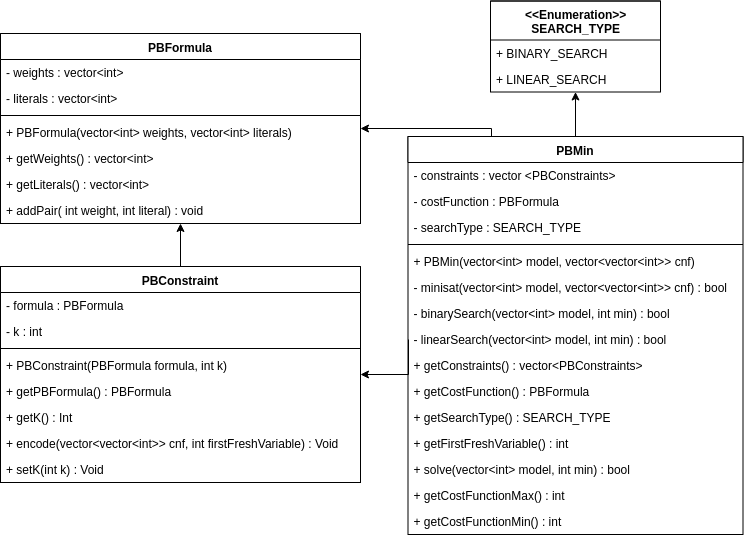
\includegraphics[width=1\textwidth]{Figures/Iteration_1_Architecture.png}
	\captionof{figure}{Iteration 1 architecture}
	\label{it1arch}
\end{center}


\paragraph{PBFormula}

This class is the one responsible for representing a Pseudo-Boolean Formula. In order to make it more interoperable with PBLib, it adopted the same representation for variables and weights which are int32\_t and int64\_t respectively.  

%TODO: it is possible to talk in more detail about it) 



\paragraph{PBConstraint} 

A Pseudo-Boolean Constraint is represented as a PBFormula and a boundary.  \\
The function \emph{encode()} is responsible for converting the Pseudo-Boolean Constraints into a CNF. This encoding is the part done with PBLib. \\
Note that there is no way of specifying the relational operator of the constraint because it will always be $\leq$.  Other constraints can be easily converted into this type as specified in \cite{Abio}.

%TODO: it is possible to talk in more detail about it) 



\paragraph{PBMin} 

This class is responsible for representing a Pseudo-Boolean Minimization problem.  It is formed by a vector of PBConstraint, the cost function which is a PBFormula and the search type which is defined by the enum \emph{SEARCH\_TYPE}.  \\
This enum has two values, \emph{BINARY\_SEARCH} and \emph{LINEAR\_SEARCH}, which are the search strategies specified in the objectives of the project.  \\\\
This class has the following methods: 
\begin{itemize}
	\item \emph{minisat()} is responsible for calling the solver, Minisat, and get the model back if it exists.
	\item \emph{binarySearch()} is responsible for executing the Binary Search algorithm to find the optimal value for the problem.
	\item \emph{linearSearch()} is responsible for executing the Linear Search algorithm to find the optimal value for the problem.
	\item \emph{getFirstFreshVarialbe()} returns a value called first fresh variable which is required by PBLib in order to encode the constraints into a CNF.
	\item \emph{solve()} is called by the user once he/she wants to solve the problem.
	\item \emph{getCostFunctionMax()} returns the maximum possible value for the cost function.
	\item \emph{getCostFunctionMin()} returns the minimum possible value for the cost function.
\end{itemize}
As the reader may have noticed, this contradicts the initial intention which was that this class should be only responsible for representing a Pseudo-Boolean Minimization problem. The methods listed above show that the class is also responsible for calling Minisat, implementing the search strategies and, as a consequence of this, calling PBLib for encoding the problem into a CNF.  

\begin{verse}
	This error in the class design had a negative impact on the next iteration which required a redesign of the architecture. It will be explained in \ref{arch-error}.
\end{verse}

\subsection{Development and TDD}

The developed started with the leaf class at the hierarchy, as seen in the architecture\ref{it1arch}, PBFormula.  \\
%TODO: Explain in more detail the development) 
Following the hierarchy, the next one was PBConstraint and the last one PBMin. \\\\
The first implemented method from PBMin was \emph{int32\_t PBMin::getFirstFreshVariable()}. This method has to return the next available literal to be used in the future by PBLib. To achieve this behaviour, this method looks at all the literals that are in the PBMin (constraints and cost function) and returns the maximum absolute literal found plus one.  \\
For example, if we have the constraint $3*1 + 2*(-2) \leq 3$, and the cost function $4*(-1) + 7*2$, the first fresh variable is 3. \\\\
The methods \emph{int64\_t PBMin::getCostFunctionMax()} and \emph{int64\_t PBMin::getCostFunctionMin()} are required to limit the search strategies. The optimal value has to be comprehended between these limits.  \\
The first part of these two methods does the same: For each literal at the cost function sums the weights where it appears positive and the weights where it appears negated and stores them in \emph{positive[i]} and \emph{negative[i]} where $i$ is the literal.\\
The maximum value for the cost function is that where a literal is set to true if \emph{positive[i]} is bigger than \emph{negative[i]}. Similarly, the minimum value for the cost function is that where a literal is set to true if \emph{negative[i]} is bigger than \emph{positive[i]}.\\\\
For example, given the cost function $-1*1 - 3*(-1) + 7*2 -5*(-2)$,\\
\emph{positive = \{-1,7\}}\\
\emph{negative = \{-3,-5\}}\\
Literal $1$ is set to $true$ because $positive[1] > negative[1]$.\\
Literal $2$ is set to $true$ because $positive[2] > negative[2]$.\\
The maximum value for the cost function is $6$.\\
Literal $1$ is set to $false$ because $positive[1] > negative[1]$.\\
Literal $2$ is set to $false$ because $positive[2] > negative[2]$.\\
The minimum value for the cost function is $-8$.\\\\
bool PBMin::binarySearch(std::vector< int32\_t > \& model, int64\_t \& min) \\
bool PBMin::linearSearch(std::vector< int32\_t > \& model, int64\_t \& min) 

\subsection{Finalization}

At this substage, some techniques learned at the Erasmus course, Software Testing, such as Category Partition Testing were applied.  \\
%TODO: At this point, Category Partition Testing should already be explained) 
These new tests revealed some bugs in the search strategies implementation for particular values for the algorithms. 

\begin{table}[h!]
	\centering
	\begin{tabular}{|l|c|c|c|}
		\hline
		\multicolumn{1}{|c|}{Class} & \emph{min} is the first value & \emph{min} is the last value & Unsatisfiable \\ \hline
		Linear Search & \begin{tabular}[c]{@{}c@{}} $\overline{x_1} \leq 0$ \\ $x_1$ \end{tabular} & \begin{tabular}[c]{@{}c@{}} $x_1 \leq 0$ \\ $x_1$\end{tabular}  & \begin{tabular}[c]{@{}c@{}} $2x_1 \leq 1$ \\ $2\overline{x_1} \leq 1$ \\ $x_1$\end{tabular} \\ \hline
		Binary Search & \begin{tabular}[c]{@{}l@{}} $\overline{x_1} \leq 0$ \\ $5x_1 + 5x_2$\end{tabular} & \begin{tabular}[c]{@{}c@{}} $\overline{x_1} \leq 0$ \\ $3x_1 + 7x_2$ \end{tabular} & \begin{tabular}[c]{@{}c@{}} $2x_1 \leq 1$ \\ $2\overline{x_1} \leq 1$ \\ $x1$\end{tabular} \\ \hline
	\end{tabular}
	\caption{Category partition testing for \emph{Linear search} and \emph{Binary search}}
	\label{cpt}
\end{table}

\section{Objective 2: Timeout}

\subsection{Problem}
It has been previously explained that SAT is an NP-Complete problem which means that there is no known algorithm which can solve it in polynomial time. In other words it can take a lot of time to solve this type of problems. \\
For example, a CNF of 300 variables and 1200 clauses takes 50 seconds to be solved.  \\\\
Some users need a result before certain time. For instance, a delivery company need a plan every morning before 08:00 AM for their trucks,packages and drivers. Therefore some users need a result before a certain time even if it is not the optimal one.  \\\\
In order that the software was able to work with this new feature, it needed a new parameter from the user and timeout strategies.

\subsection{Possible solutions}
Two different timeout strategies were considered:  

\begin{itemize}
	\item A maximum number of seconds for each call to the solver.
	\item A maximum number of seconds for the whole problem. 
\end{itemize}
Both options were considered useful, and hence they become a goal for the development substage.   

\subsection{Planning}
Some research was done about timeout strategies for solvers.  \\
%TODO: Explain sat solvers resets) 
In order to implement the asynchronous behaviour two different approaches were considered:  

\paragraph{Threads}

Threads within the same process can communicate using shared memory. \\
Threads share the same memory space which could be a source of problems if not handled carefully. In this particular case, this is helpful because the thread would execute the solver call while the parent is waiting for the timeout.  

\paragraph{Processes}

Child processes are easier to work with but, in general, they are more expensive. This is because processes have their own code, memory space, files, registers and stack which implies that every time a new child process is created, some of the listed elements need to be copied.  \\\\\\\\
Finally, Threads was the chosen option because of the following reasons: 

\begin{itemize}
	\item They sharer memory within a process which makes communication much more manageable. In this particular project, this allowed the code to be more simple. 
	\item They are less expensive to create because no copy of memory is effectuated.
\end{itemize}
The timeout was thought to be implemented as a signal sent from the parent thread to the child thread.  


\paragraph{What happens when there is a timeout?\\}
The answer depends on the timeout strategy selected for the problem: \emph{GeneralTimeoutSolver} or \emph{SimpleTimeoutSolver}. \\\\
In the first case, the flag \emph{timeoutOccurred} is set to \emph{true}, and the last found solution is returned. With the flag, the user can know if the timeout occurred and therefore know the solution may not be optimal.  \\
In the second case, the flag \emph{timeoutOccurred} is also set to \emph{true} and the current solver execution is killed. However, the search algorithm will keep running with the next values.  
\begin{center}
	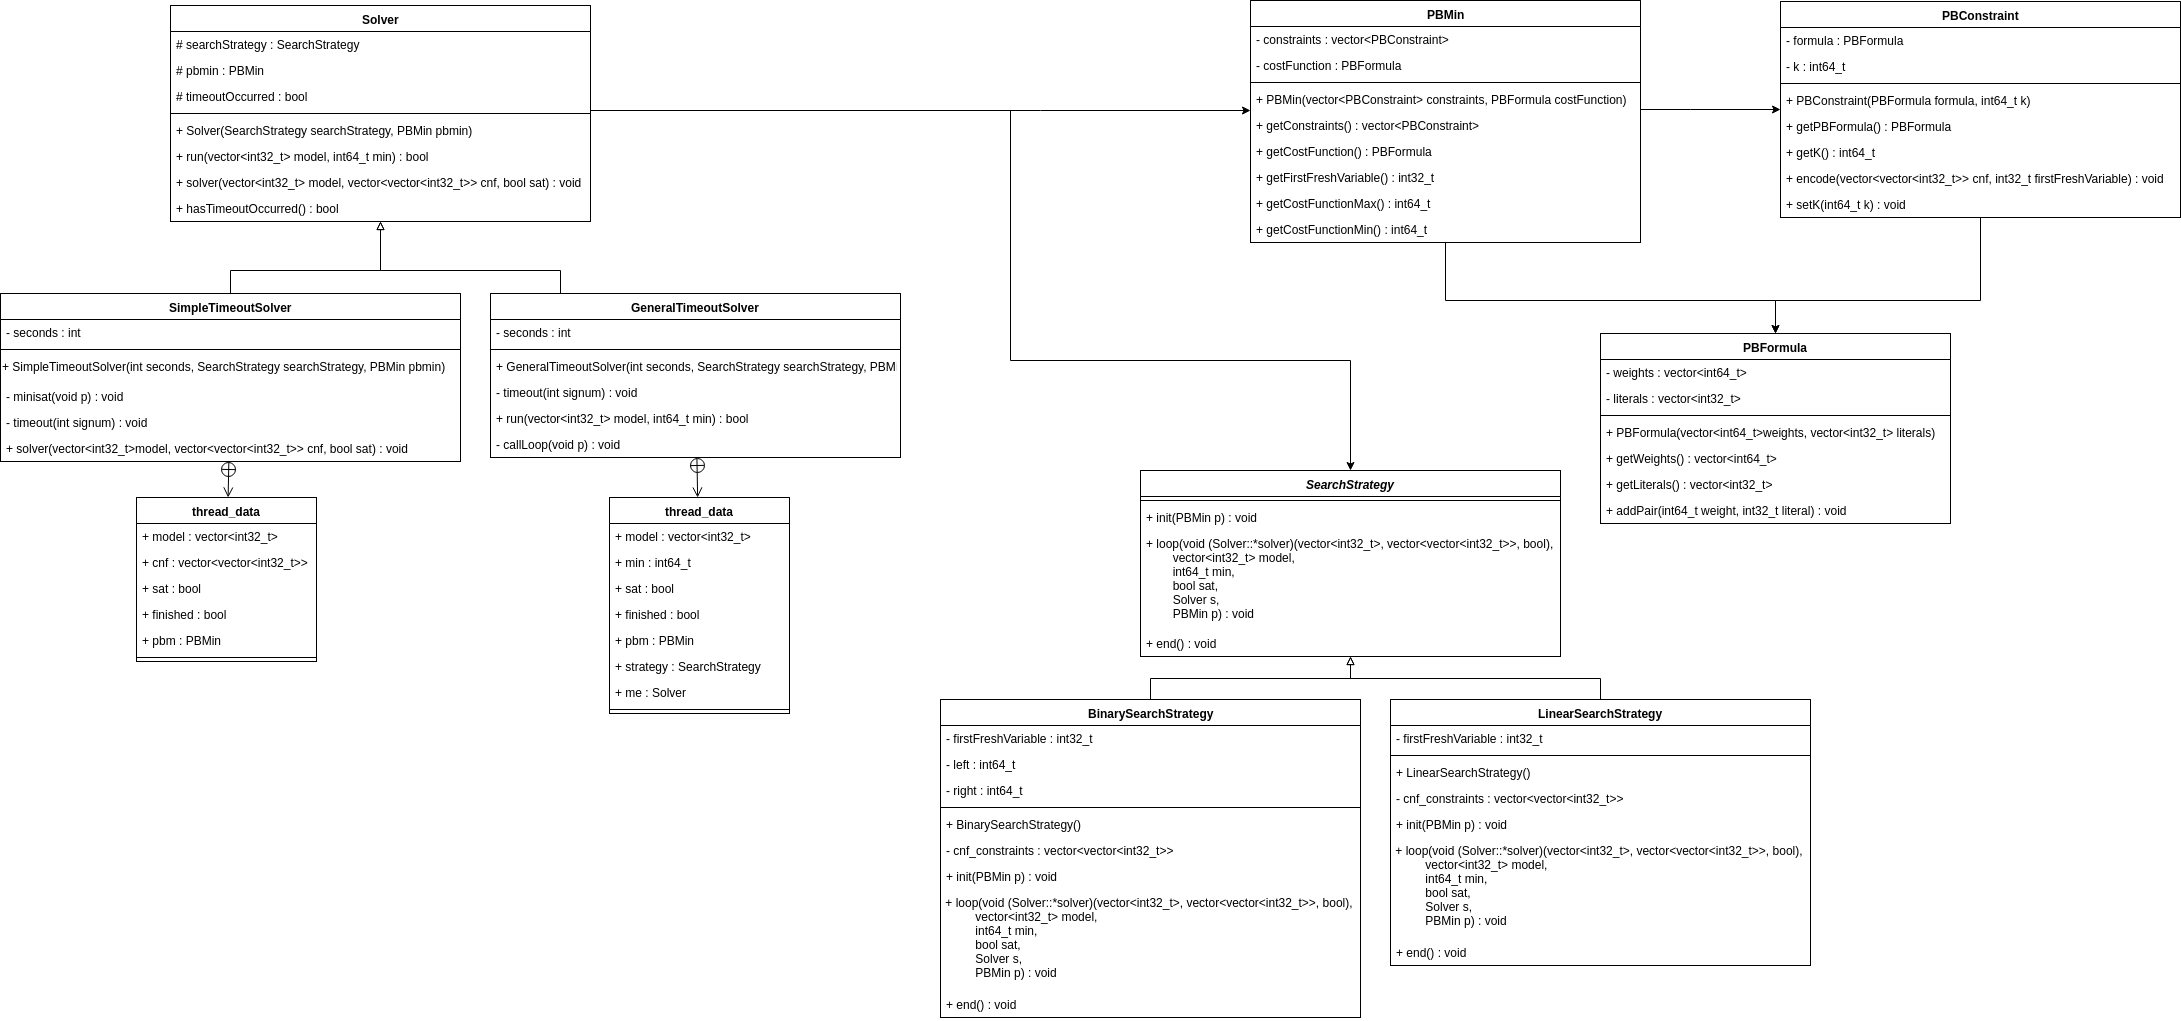
\includegraphics[width=1.6\textwidth, angle=90]{Figures/Iteration_2_Architecture-UML.png}
	\captionof{figure}{Iteration 2 architecture}
	\label{it2arch}
\end{center}
\label{arch-error}
As can be seen, the architecture suffered an evolution from the previous iteration. As previously mentioned in Iteration 1, the class PBMin was not respecting the Single responsibility principle because apart from representing the problem, it also was responsible for implementing the search strategies, calling PBLib encodings, \ldots \\ 
That architecture would have resulted in a much complex PBMin class because it would have to be responsible for the timeouts.  \\\\
For these reasons the following classes were modified or added: 
\begin{itemize}
	\item PBMin : After the refactor, this class is only responsible for representing a Pseudo-boolean minimization problem which was its original mission.
	\item SearchStrategy : One of the functionalities moved outside the PBMin class was the search strategy selection and implementation which needed to be moved to another class. For that reason, a new hierarchy of classes was created: SearchStrategy, BinarySearchStrategy and LinearSearchStrategy.  These set of classes have three methods: 
	\begin{itemize}
		\item \emph{init()}'s purpose is to prepare the class for the execution of the search algorithm. For example, encode the PBConstraints   into a CNF. 
		\item \emph{loop()}'s purpose is to execute the search algorithm.  
		\item \emph{end()} is executed after the loop once the optimal solution is found, there is no solution or a timeout occurred. It has no use by default.  
	\end{itemize}
	\item \emph{BinarySearchStrategy} uses the \emph{loop()} method to implement the binary search algorithm. 
	\item \emph{LinearSearchStrategy} uses the \emph{loop()} method to implement the linear search algorithm. 
	\item \emph{Solver} : Another behaviour removed from the PBMin class is the actual execution of the problem solver. This behaviour was moved to a new class, Solver, which is responsible for calling the SAT solver. This class is the solver without a timeout, that it is implemented by its children SimpleTimeoutSolver and GeneralTimeoutSolver. The main methods are: 
	\begin{itemize}
		\item \emph{run()} is the function called by the user once he/she wants to solve the problem.
		\item \emph{solve()} is responsible for calling the SAT solver, passing the CNF and getting back the result. 
	\end{itemize}
	\item \emph{SimpleTimeoutSolver} overrides the method \emph{solve()} and adds the creation of a thread which calls the solver while it counts for the timeout.  
	\item \emph{GeneralTimeoutSolver} overrides the method \emph{run()} and adds the creation of a thread which calls the selected search algorithm while it counts for the timeout. 
\end{itemize}  

\subsection{Development and TDD}
The first thing to do was refactor the class PBMin and move all the functionalities previously mentioned to the new classes. This also implied a refactor to the PBMin tests. Like the previous iteration, the development was done selecting classes in a bottom-up way.  \\\\
The first class created was Solver which does not implement a timeout strategy. Therefore it has the same functionality as the old PBMin: call the search algorithm and the SAT solver. As seen in the architecture diagram \ref{it2arch} this class has a dependency in the \emph{SearchStrategy} class which was not implemented at that time. To apply TDD methodology, it was necessary to create a stub. As a stub, the only purpose of \emph{SearchStrategy\_Stub} was to implement a fake behaviour in order to test the Solver class. \\
The next implemented classes were \emph{SearchStrategy}, \emph{BinarySearchStrategy} and \emph{LinearSearchStrategy} hierarchy.  \\\\
\emph{SearchStrategy} is an abstract class which means it cannot be instantiated. Its purpose is to be a "contract" between search strategies, such as linear search and binary search, and classes which use them. Because it has no code, it is not necessary to be tested.  \\
However, for its children it is mandatory. The first child, \emph{LinearSearch} implements the linear search algorithm which was in the old PBMin class. The method \emph{init()} encodes the PBConstraints of the problem into a CNF. This encoding is done at the \emph{init()} method because it has to be done only once.  \\
The method \emph{loop()} is the one which implements the algorithm. It starts defining the boundaries of the search with the maximum possible value for the cost function and its minimum.  \\
Because of the values given by the algorithm only differ in one unit, starting on the maximum and ending on the minimum, the functionality "Incremental constraints" from PBLib could be used.\\ %TODO: Explain incremental constraints PBLib)  
Finally, the method \emph{end()} does nothing. \\
The other child, \emph{BinarySearchSolver}, implements the binary search algorithm. As before, the method \emph{init()} encodes the problem constraints into a CNF. The \emph{loop()} method implements the binary search algorithm taking as the left value the minimum possible value of the cost function and as the right value its maximum. Unlike before, the incremental constraints functionality could not be used because the search is not "constant".  Finally, as before, the method \emph{end()} does nothing.  \\\\
Finally, the last classes to be implemented were \emph{SimpleTimeoutSolver} and \emph{GeneralTimeoutSolver}. \\
The Template pattern \cite{Gamma} could be applied because the children of \emph{Solver} are a specialization of it. In other words, all the hierarchy shares a lot of behaviour.  \\
The \emph{SimpleTimeoutSolver} only redefines the method \emph{solve()} to a creation of a thread which calls the sat solver with all its implications. \\
The \emph{GeneralTimeoutSolver} only redefines the method \emph{run()} to a creation of a thread which calls the function \emph{loop()} from the \emph{SearchStrategy} class.  

\subsection{Finalization}
The classes \emph{Solver}, \emph{SimpleTimeoutSolver} and \emph{GeneralTimeoutSolver}, apart from their unit tests required by TDD, were tested with integration tests.  \\
%\begin{table}[h!]
%	\centering
%	\begin{tabular}{l|l|l|l|}
%		\cline{2-4}
%		\multicolumn{1}{c|}{} & \multicolumn{1}{c|}{BinarySearchStrategy} & \multicolumn{1}{c|}{LinearSearchStrategy} & SlowSearchStrategy \\ \hline
%		\multicolumn{1}{|l|}{Solver} & Solver\_BinarySearchStrategy\_INT & Solver\_LinearSearchStrategy\_INT &  \\ \hline
%		\multicolumn{1}{|l|}{SimpleTimeoutSolver} & \begin{tabular}[c]{@{}c@{}} SimpleTimeoutSolver\_\\ BinarySearchStrategy\_INT \end{tabular} & \begin{tabular}[c]{@{}c@{}} SimpleTimeoutSolver\_ \\ LinearSearchStrategy\_INT \end{tabular}  &  \\ \hline
%		\multicolumn{1}{|l|}{GeneralTimeoutSolver} & \begin{tabular}[c]{@{}c@{}} GeneralTimeoutSolver\_ \\ BinarySearchStrategy\_INT  \end{tabular}  & \begin{tabular}[c]{@{}c@{}} GeneralTimeoutSolver\_ \\ LinearSearchStrategy\_INT \end{tabular}  & GeneralTimeoutSolver\_SlowSearchStrategy\_INT \\ \hline
%	\end{tabular}
%	\caption{Integration tests combination}
%	\label{integration-tests-combination}
%\end{table}
Integration testing was done to expose defects in the communication of classes and also test the \emph{Solver} hierarchy with real implementations of \emph{SearchStrategy} and see that the timeout was working as expected. 
